\chapter{Interaktion}
Um aus der Visualisierung ausgewählter Strukturen und Informationen eine interaktive Projektion zu erzeugen ist es erforderlich Benutzereingaben zu erfassen und auszuwerten. Die in diesem Kapitel beschriebene Interaktion ermöglicht dem Benutzer die Projektion und die damit gekoppelten Modelldaten zu modifizieren.

\section{Detektion der Benutzerinteraktion}
Für die Erkennung der Benutzereingaben werden die durch die Kinect gewonnenen Tiefeninformationen in Form der erzeugten Punktwolken ausgewertet. Während der Benutzer das \kps{} in der einen Hand hält, kann die andere Hand verwendet werden um mit der Projektion zu interagieren. Darüber hinaus können auch weitere Benutzer mit dem System interagieren.\\
%PreviewVersion
%\red[sofern sie bei der Benutzereingabe die Rahmenbedingungen der Funktionsweise beachten].\\

Der implementierte Interaktionsansatz basiert auf der Analogie zu einem Laserpointer. Ziel ist es, dem Benutzer durch Zeigebewegungen die Interaktion mit der projizierten Modellumgebung zu ermöglichen.\\
Innerhalb des Softwaremoduls \textit{Interaktion} (\kapitel{chap.softwarestruct}) erfolgt dafür zunächst eine Distanz-Filterung der Punktwolke, da weit entfernte Messpunkte nicht aus der Benutzereingabe stammen können, sondern die Umgebung abbilden. Alle Punkte außerhalb dieses Bereiches können für die weiteren Betrachtungen somit verworfen werden. Es ergibt sich damit der für die Benutzereingabe zur Verfügung stehende Interaktionsbereich, welcher in \abb{fig.intfov} dargestellt ist.\\
%\red[xmin durch Hardware gegeben, Bereich dann parametrierbar, alles darüber (rot) wird verworfen\\]

\begin{figure}[!ht]
	\begin{center}
		\includesvgnew[1]{images/interaktionsbereich_scaled}%
%		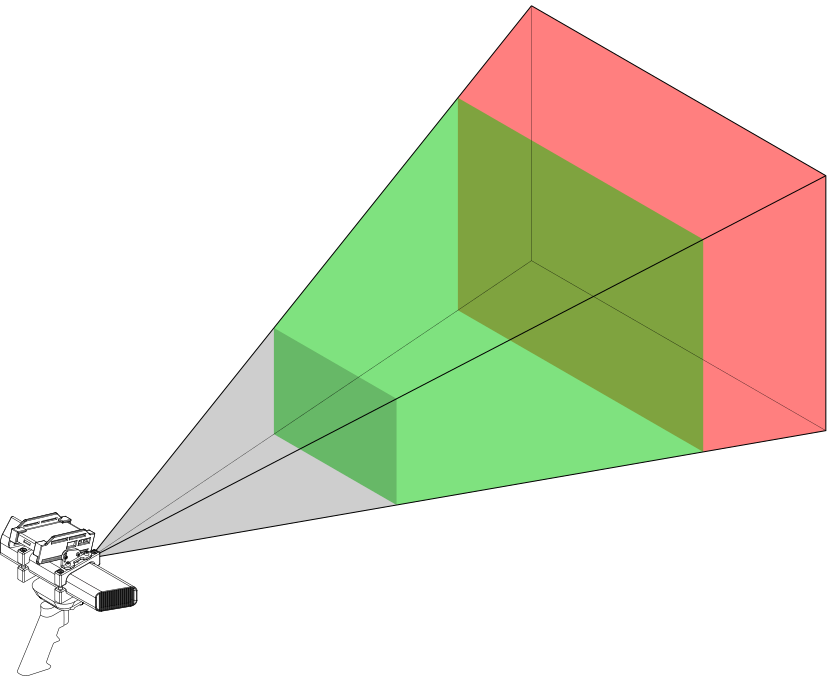
\includegraphics[scale=0.4]{interaktionsbereich}
		\caption{Parametrierbarer Interaktionsbereich}
		\label{fig.intfov}
	\end{center}
	%\vspace*{-8mm}
\end{figure}

%PreviewVersion
%\red[Bemaßung!\\]
Der minimale Abstand $z_{min}$ beträgt \SI{0,5}{\meter} und wird durch die Spezifikationen der Kinect definiert. Der maximale Interaktionsabstand $z_{int}$ ist parametrierbar und kann damit anwendungsspezifisch definiert werden.\\

Basierend auf den nach der Filterung verbleibenden Punkte wird eine Ebenendetektion nach \cite{Fischler1981} durchgeführt. Alle Punkte innerhalb eines definierten Abstandes werden daraufhin auf die ermittelte Ebene projiziert, wodurch eine zweidimensionale Abbildung erzeugt und Messwertrauschen geglättet wird. Außerhalb der Ebene liegende Punkte werden für die weiteren Schritte aus der Betrachtung entfernt. Dazu gehören deutliche Ausreißer innerhalb der detektierten Interaktionsstruktur sowie weitere Artefakte in der Punktwolke.\\

Um eine gleichmäßige Objektstruktur zu erhalten wird anschließend eine Hüllkurve um die verbleibenden Punkte gelegt und die vorhandene Struktur mittels einer äquidistanten Verteilung von Punkten angenähert. Aus dieser Hüllkurve wird der geometrische Schwerpunkt (Basis) sowie der vom \kps{} am weitesten entfernte Punkt (Spitze) bestimmt. Der Verbindungsvektor zwischen Basis und Spitze bildet damit die Zeigerichtung des Anwenders ab. Der gesamte Ablauf zur Bestimmung der Zeigerichtung ist in \abb{fig.intdir} dargestellt.\\

\begin{figure}[!ht]
	\begin{center}
	\subfigure[Ausschnitt aus vollständiger Punktwolke]{
		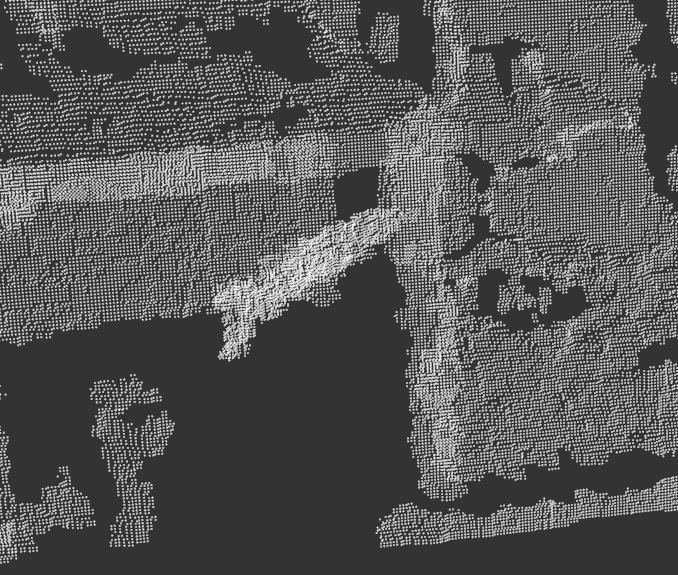
\includegraphics[width=5cm]{interaction_01_02}
	}
	\hspace{5mm}
	\subfigure[Gefilterte Interaktionsstruktur abgebildet auf detektierte Ebene]{
		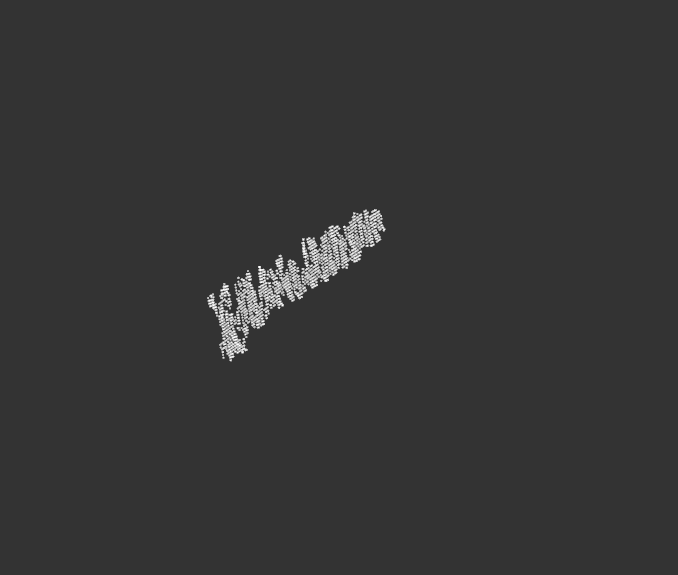
\includegraphics[width=5cm]{interaction_02_02}
	}
		\subfigure[Hüllkurve und geometrischer Schwerpunkt der Struktur]{
		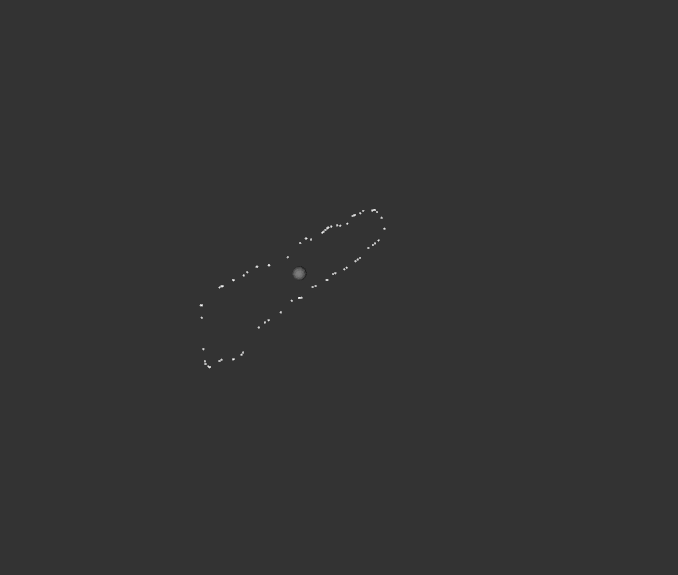
\includegraphics[width=5cm]{interaction_03_02}
	}
	\hspace{5mm}
	\subfigure[Zeigerichtung definiert durch Verbindung zwischen Basis und Spitze]{
		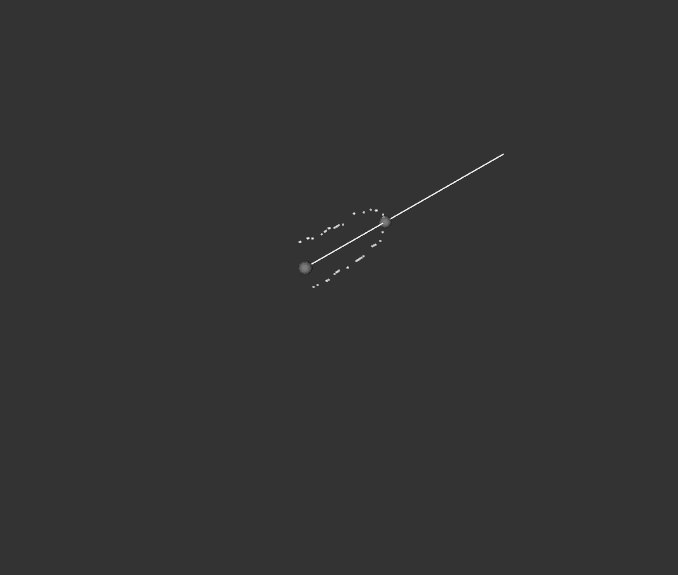
\includegraphics[width=5cm]{interaction_04_02}
	}
	\caption{Filterung der Punktwolke zur Bestimmung der Zeigerichtung}
	\label{fig.intdir}
	\end{center}
	%\vspace*{-8mm}
\end{figure}

Um das Signal der ermittelte Linie zu glätten wird der gleitende Mittelwert der Punkte bestimmt. Auch die Differenz zwischen zwei Punkten aus aufeinander folgenden Messungen wird überwacht, um Sprünge in der Bewegung aufgrund von Fehldetektionen erkennen zu können.\\
Aufgrund des Implementierten Ansatzes wurde für die Kommunikation eine Nachrichtenstruktur definiert, welche die erkannte Linie abbildet. Das Modul \textit{Interaktion} stellt die ermittelte Linie über diese Nachricht zur Verfügung, so dass sie vom Modul \textit{Visualisierung} ausgewertet werden kann.\\

%Da die Kamera des Kinect Sensors auch von dem \mFovis verwendet wird besteht die Gefahr der Beeinflussung zwischen der Benutzereingabe und der lokalen Lokalisation. Um diese zu vermeiden sendet das \mInteraction Modul einen Befehl zum Pausieren der visuellen Odometrie sobald Punkte innerhalb des Interaktionsbereiches erkannt werden. Die visuelle Odometrie wird somit für die Dauer der Benutzerinteraktion unterbrochen. Sobald keine Punkte mehr innerhalb des Interaktionsbereiches detektiert werden, sendet das \mInteraction ein Signal zur Wiederaufnahme der visuellen Odometrie an das \mFovis .
Da die Kamera der Kinect auch zur Bestimmung der visuellen Odometrie verwendet wird besteht die Gefahr, dass die lokale Lokalisation durch die Benutzereingabe beeinträchtigt wird. Um dies zu vermeiden wurde eine direkte Kommunikation zwischen den beteiligten Modulen implementiert. Die visuelle Odometrie wird dabei unterbrochen, sobald Punkte innerhalb des Interaktionsbereiches erkannt werden. Endet die Interaktion, kann die visuelle Odometrie wieder aufgenommen werden.\\
Im Falle kleiner Posenänderungen während der Benutzereingabe ist die Lokalisation in der Lage die Veränderungen zu erkennen und die Pose im Anschluss an die Benutzerinteraktion zu aktualisieren. Da das Projektionsfeld während der Interaktion jedoch ohnehin auf das ausgewählte Objekt ausgerichtet werden sollte, ist der Bewegungsraum des \kps{s} bereits aufgrund des Interaktionsverfahrens limitiert.\\

\section{Erkennung von Befehlen}
Die Auswertung der auf Basis der Zeigebewegung ermittelten Linie erfolgt innerhalb des Moduls \textit{Visualisierung}. Die Detektion der Linie erfolgte im Koordinatensystem der Kamera $\ks{K}$, so dass diese für die Auswertung zunächst über $\tmat{M}{K}$ in das Koordinatensystem der Karte $\ks{M}$ transformiert wird.\\

Um zu determinieren auf welches Modellobjekt der Benutzer gezeigt hat werden entlang der Linie alle Schnittpunkte mit den virtuellen Modelldaten bestimmt. Dazu wird die Visualisierungsumgebung VTK verwendet, welche die Ermittlung von Schnittpunkten zwischen den Modellobjekten und Linien als Funktion zur Verfügung stellt. Aus den Schnittpunkten kann somit ermittelt werden, welches Objekt der Benutzer ausgewählt hat. Um die Auswahl eines Objektes, analog einer \glqq Klick\grqq -Aktion, zu ermöglichen wurden zwei Verfahren implementiert.\\
Die erste Implementierung erfolgt durch Überprüfung der Verweildauer des simulierten Zeigers auf dem Objekt. Überschreitet diese einen definierten Grenzwert wird dies als Auswahlbefehl gewertet und das Objekt in den Zustand \textit{aktiv} versetzt.\\
Für das zweite Verfahren wurde die Software des Arduino um einen zusätzliche Schnittstelle erweitert. Durch die Anbindung eines Tasters wird die Möglichkeit einer echten \glqq Klick\grqq -Aktion zur Befehlseingabe realisiert.
%PreviewVersion
%\red[Oder im Ausblick aufführen?\\]

Durch Veränderung der Textur erhält der Anwender wie in \abb{fig.intintersect} dargestellt das visuelle Feedback, dass ein Objekt ausgewählt und in den neuen Status versetzt wurde.

\begin{figure}[!ht]
	\begin{center}
	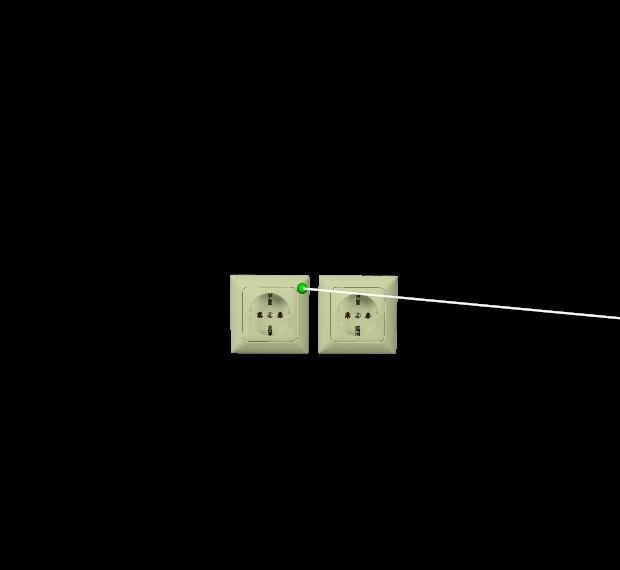
\includegraphics[width=5cm]{model_selection_02}
	\caption{Auswahl eines Modellobjekts durch den Benutzer}
	\label{fig.intintersect}
	\end{center}
	%\vspace*{-8mm}
\end{figure}

%\begin{figure}[!ht]
%	\begin{center}
%		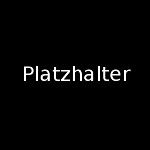
\includegraphics[scale=1.0]{spacer}
%		\caption{Subfigures: Line intersection mit Modell und Abbildung des Laserpunktes - Aktivierung des Objektes}
%		\label{fig.intintersect}
%	\end{center}
%	%\vspace*{-8mm}
%\end{figure} 

Innerhalb der Modellumgebung können nun temporäre Interaktionsobjekte wie in \abb{fig.intarrows} (a) dargestellt eingeblendet werden, welche vom Benutzer ebenfalls über das zuvor beschriebene Funktionsprinzip ausgewählt werden können. Alle weiteren Modellobjekte werden während dieser Phase in den Status \textit{inaktiv} versetzt. Es ist somit immer nur ein Objekt der virtuellen Umgebung \textit{aktiv}, wodurch für den Anwender eine klare Zuordnung der Interaktionsobjekte möglich ist.

\begin{figure}[!ht]
	\begin{center}
	\subfigure[Auswahl eines temporären Interaktionsobjektes]{
		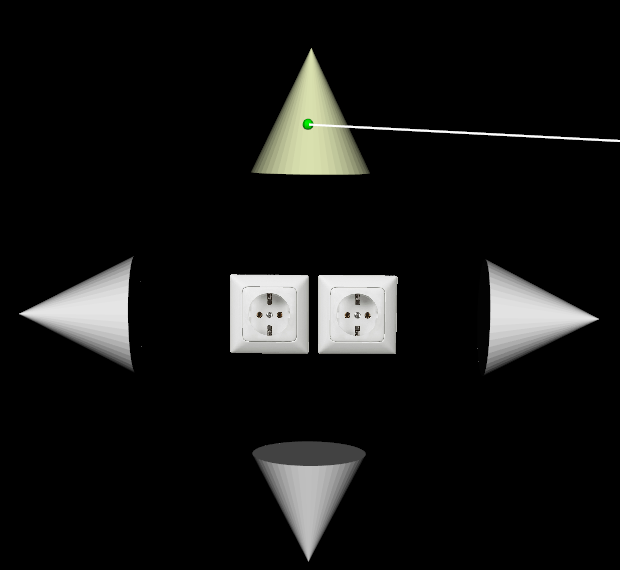
\includegraphics[width=5cm]{model_selection_04}
	}
	\hspace{5mm}
	\subfigure[Bewegtes Modellobjekt mit aktualisierten Interaktionsobjekten]{
		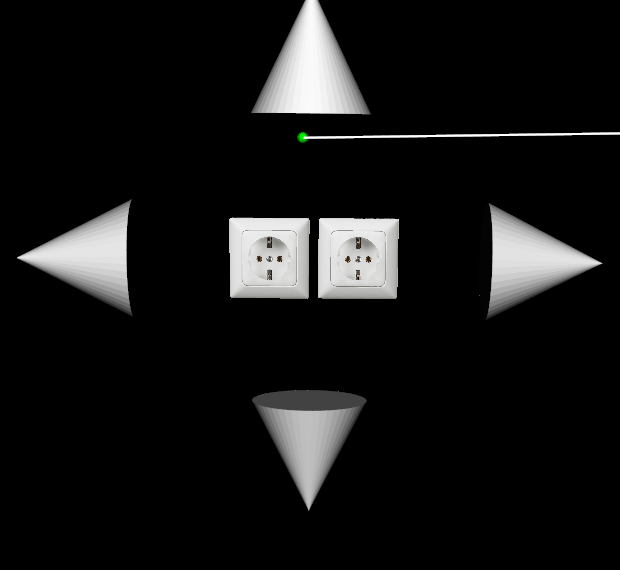
\includegraphics[width=5cm]{model_selection_05}
	}
	\caption{Modifikation der Pose eines Modellobjektes durch Auswahl eines Interaktionsobjektes}
	\label{fig.intarrows}
	\end{center}
	%\vspace*{-8mm}
\end{figure}

Durch Auswahl der Interaktionsobjekte ist der Benutzer in der Lage das aktuell als \textit{aktiv} gewählte Objekt innerhalb der Modellumgebung zu modifizieren. \abb{fig.intarrows} (b) zeigt dies am Beispiel der Translation des Modellobjektes. Die Anzahl und Funktion der Interaktionsobjekte kann dabei je nach Anwendungsfall spezifiziert werden, so dass eine Modifikation der Objekte bezüglich aller sechs räumlichen Freiheitsgrade möglich ist.\\

Durch die Erkennung der Benutzereingabe können somit Objekte der Modellumgebung ausgewählt und bezüglich ihrer Pose modifiziert werden. Die Integration der Interaktion in die Visualisierung ermöglicht die direkte Modifikation der zugrunde liegenden Modelldaten. Das aktualisierte Modell kann abschließend gesichert werden wodurch eine Rückführung in den virtuellen Modellierungs- und Planungsprozess erreicht wird.

%PreviewVersion
%\red[Intersection sollte auch mit Modellumgebung möglich sein, damit der Pointer realistisch abgebildet wird!? Vielleicht Modell (obj) der Karte mit schwarzer Textur?]